


%
% Deuteron: quark ornac-pairs with ornac axis
%
\begin{wrapfigure}{r}{0.5\textwidth}
  \begin{center}
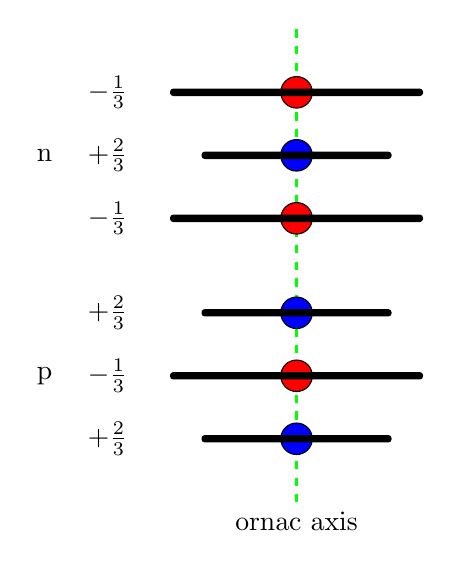
\begin{tikzpicture}[scale=0.4, rotate=0]



% Ornac axis
\draw[green, dashed, very thick] (4,4) -- (4,-11) ;
\path 
(4,-11) node [below]  {ornac axis};

%
% Neutron
%
\path 
(-4,0) node   {n};


% Down quark ornac-pair
\path 
(-2,2) node  (red) {$-\frac{1}{3}$};

\filldraw[fill=red, draw=black] (4,2) circle [radius=0.5];

\filldraw[fill=black, draw=black ,rounded corners=1pt] (0, 1.9) rectangle (8, 2.1);


% Up quark ornac-pair
\path 
(-2,0) node  (red) {$+\frac{2}{3}$};

\filldraw[fill=blue, draw=black] (4,0) circle [radius=0.5];

\filldraw[fill=black, draw=black ,rounded corners=1pt] (1,-0.1) rectangle (7, 0.1);



% Down quark ornac-pair
\path 
(-2,-2) node  (red) {$-\frac{1}{3}$};

\filldraw[fill=red, draw=black] (4,-2) circle [radius=0.5];

\filldraw[fill=black, draw=black ,rounded corners=1pt] (0, -1.9) rectangle (8, -2.1);


%
% Proton
%

\path 
(-4,-7) node   {p};

% Up quark ornac-pair
\path 
(-2,-5) node  (red) {$+\frac{2}{3}$};

\filldraw[fill=blue, draw=black] (4,-5) circle [radius=0.5];

\filldraw[fill=black, draw=black ,rounded corners=1pt] (1, -4.9) rectangle (7, -5.1);



% Down quark ornac-pair
\path 
(-2,-7) node  (red) {$-\frac{1}{3}$};

\filldraw[fill=red, draw=black] (4,-7) circle [radius=0.5];

\filldraw[fill=black, draw=black ,rounded corners=1pt] (0, -6.9) rectangle (8, -7.1);


% Up quark ornac-pair
\path 
(-2, -9) node  (red) {$+\frac{2}{3}$};

\filldraw[fill=blue, draw=black] (4,-9) circle [radius=0.5];

\filldraw[fill=black, draw=black ,rounded corners=1pt] (1,-8.9) rectangle (7, -9.1);



\end{tikzpicture}
\end{center}
\caption{Deuteron from side build up off quark ornac-pairs with ornac axis
\label{fig:Deuteron from side build up off quark ornac-pairs}}
\end{wrapfigure}

% End Deuteron




